\documentclass[border=10pt]{standalone}

\usepackage{tikz}
\usepackage{tikzsymbols}
\usetikzlibrary{calc,patterns,shapes.geometric}

\def\centerarc[#1](#2)(#3:#4:#5){\draw[#1] ($(#2)+({#5*cos(#3)},{#5*sin(#3)})$) arc (#3:#4:#5);}

\begin{document}
	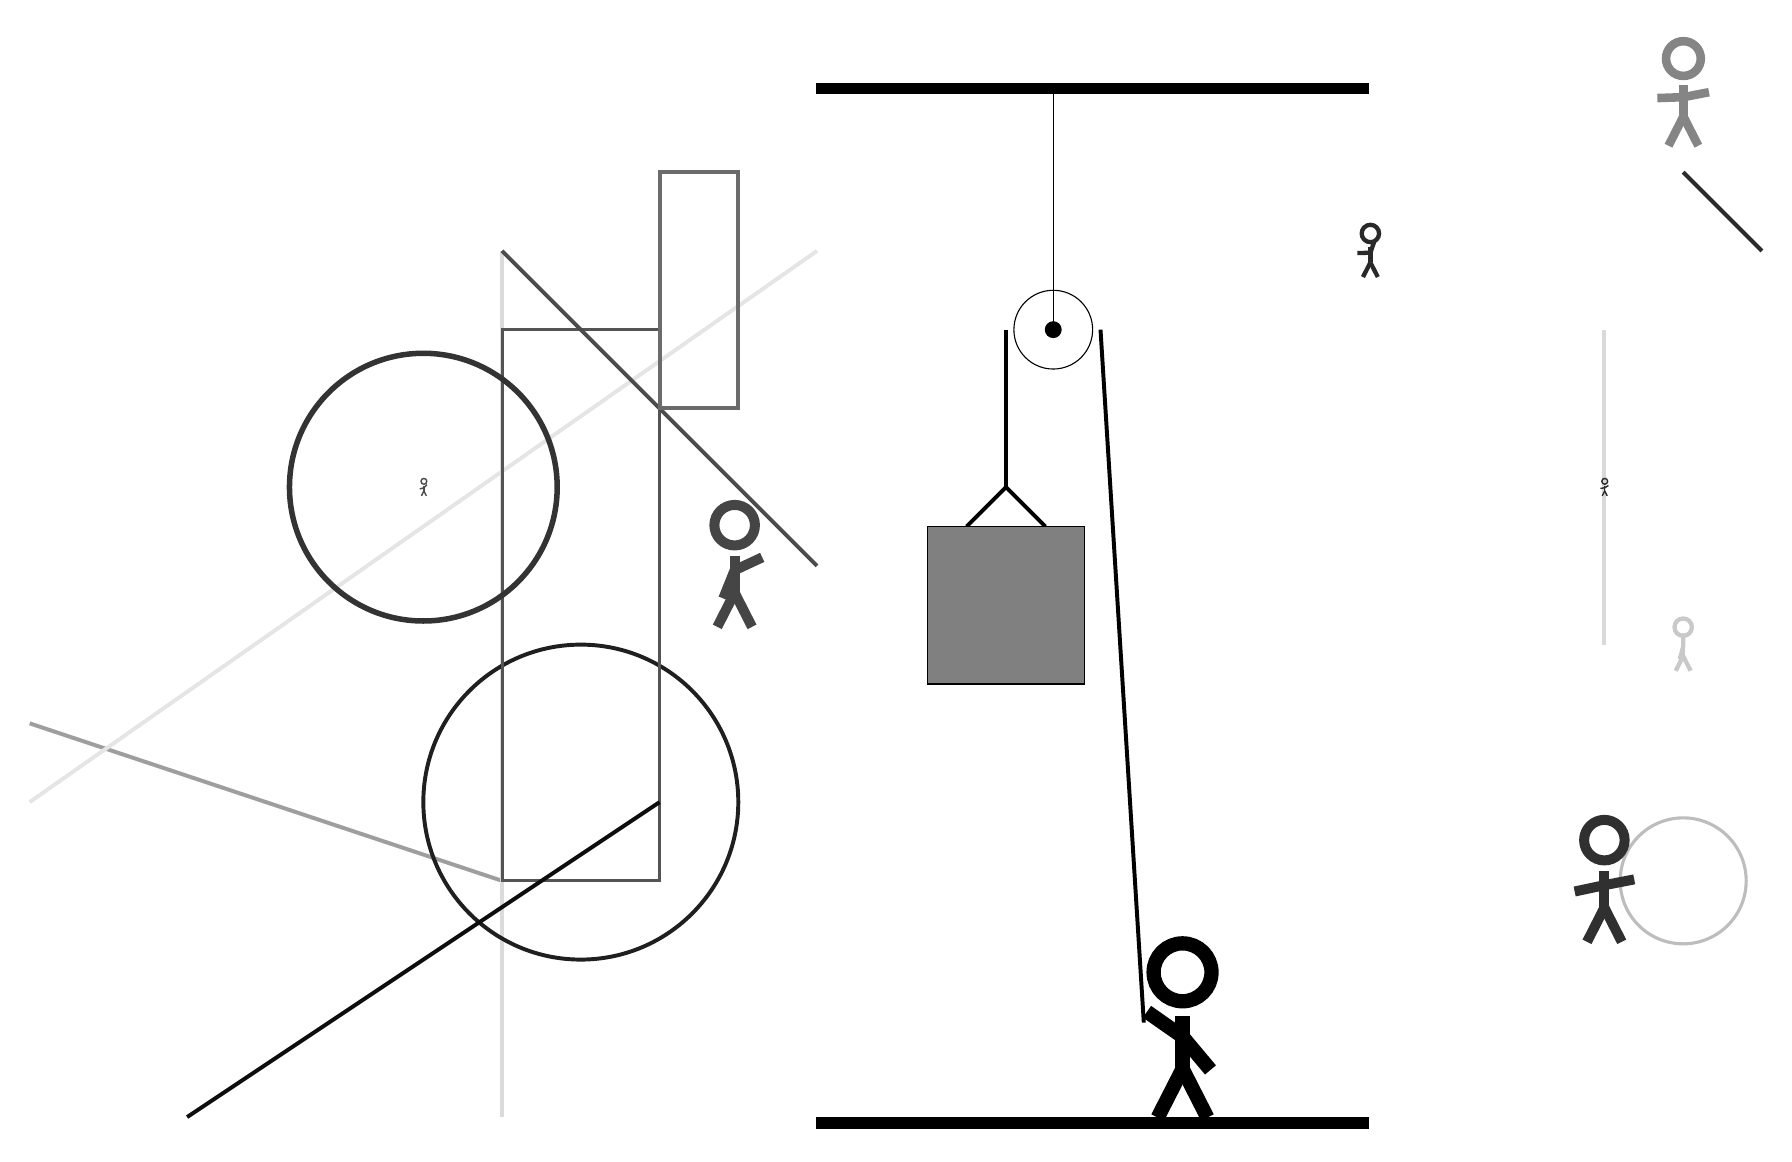
\begin{tikzpicture}
		%%%%% START %%%%%
		
		\draw[fill=black] (-2, 10) rectangle (5, 10.125);
		
		\draw (1, 7) circle (0.5);
		\draw[fill=black] (1, 7) circle (0.1);
		\draw (1, 10) -- (1, 7);
		
		\draw[line width=0.5mm] (-0.1, 4.5) -- (0.4, 5.0) -- (0.9, 4.5);
		\draw[fill=black!50] (-0.6, 4.5) rectangle (1.4, 2.5);
		
		\draw[line width=0.5mm] (0.4, 7) -- (0.4, 5.0);
		\centerarc[line width=0.5mm](1, 7)(0:180:0.6);
		\draw[line width=0.5mm](1.6, 7) -- (2.15, -1.8);
		
		\draw[line width=0.5mm, color=black!38](-6, 0) -- (-12, 2);
		
		\draw[line width=0.5mm, color=black!10](-2, 8) -- (-12, 1);
		\draw[line width=0.5mm, color=black!14](-6, 8) -- (-6, -3);
		\draw[line width=0.5mm, color=black!83](10, 8) -- (9, 9);
		\draw [line width=0.5mm, color=black!88](-5, 1) circle (2.0);
		
		\node[line width=0.7mm, color=black!73] at (-3, 4) {\Strichmaxerl[7][68][25]};
		\node[line width=0.5mm, color=black!21] at (9, 3) {\Strichmaxerl[3][75][89]};
		\draw[line width=0.4mm, color=black!67] (-4, 0) rectangle (-6, 7);
		\draw[line width=0.5mm, color=black!15](8, 7) -- (8, 3);
		\node[line width=0.4mm, color=black!83] at (8, 5) {\Strichmaxerl[1][9][31]};
		
		\node[line width=0.5mm, color=black!70] at (-7, 5) {\Strichmaxerl[1][16][45]};
		\draw[line width=0.5mm, color=black!95](-4, 1) -- (-10, -3);
		\draw [line width=0.4mm, color=black!26](9, 0) circle (0.8);
		
		\draw[line width=0.5mm, color=black!70](-6, 8) -- (-2, 4);
		\node[line width=0.5mm, color=black!81] at (8, 0) {\Strichmaxerl[7][12][11]};
		\draw [line width=0.7mm, color=black!80](-7, 5) circle (1.7);
		
		\draw[line width=0.5mm, color=black!58] (-4, 9) rectangle (-3, 6);
		
		\node[line width=0.5mm, color=black!48] at (9, 10) {\Strichmaxerl[6][2][11]};
		\node[line width=0.6mm, color=black!84] at (5, 8) {\Strichmaxerl[3][1][71]};
		
		\node at (2.6, -1.9) {\Strichmaxerl[10][-35][-50]};
		
		\draw[fill=black] (-2, -3) rectangle (5, -3.15);
		
		%%%%% END %%%%%
	\end{tikzpicture}
\end{document}